\ifdefined\IncludeOlly
% it's not possible to slice Olly part from this example...
\chapter{\RU{Числа Фибоначчи}\EN{Fibonacci numbers}}

\RU{Еще один часто используемый пример в учебниках по программированию это рекурсивная функция,
генерирующая числа Фибоначчи}
\EN{Another widespread example used in programming textbooks is a recursive function 
that generates the Fibonacci numbers}\footnote{\url{http://go.yurichev.com/17332}}.
\RU{Последовательность очень простая: каждое следующее число\EMDASH{}это сумма двух предыдущих}\EN{The 
sequence is very simple: each consecutive number is the sum of the previous two}.
\RU{Первые два числа\EMDASH{}это единицы или 0, 1 и 1}\EN{The first two numbers are 1's or 0, 1 and 1}.

\RU{Начало последовательности}\EN{The sequence starts like this}:

\begin{center}
$0, 1, 1, 2, 3, 5, 8, 13, 21, 34, 55, 89, 144, 233, 377, 610, 987, 1597, 2584, 4181 ...$
\end{center}

\section{\RU{Пример}\EN{Example} \#1}

\RU{Реализация проста. Эта программа генерирует последовательность вплоть до}
\EN{The implementation is simple. This program generates the sequence until} 21.

\lstinputlisting{\CURPATH/fib.c}

\lstinputlisting[caption=MSVC 2010 x86]{\CURPATH/fib.asm}

\RU{Этим я хотел проиллюстрировать стековые фреймы}\EN{I want to illustrate 
the stack frames with this}.

\clearpage
\RU{Загрузим пример в \olly и дотрассируем до самого последнего вызова функции \ttf{}}
\EN{Let's load the example in \olly and trace to the last call of \ttf{}}:

\begin{figure}[H]
\centering
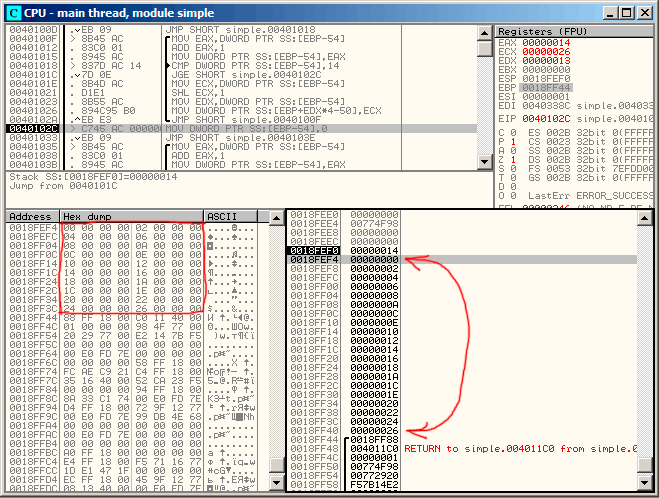
\includegraphics[scale=\FigScale]{\CURPATH/olly.png}
\caption{\olly: \RU{последний вызов \ttf{}}\EN{last call of \ttf{}}}
\label{fig:fib_olly}
\end{figure}

\clearpage
\RU{Исследуем стек более пристально}\EN{Let's investigate the stack more closely}. 
\RU{Я добавил здесь комментариев}\EN{I have added some comments to it}
\footnote{\EN{By the way, it's possible to select several entries in \olly and copy them to the clipboard (Ctrl-C).
That's what I just did.}\RU{Кстати, в \olly можно отметить несколько элементов и скопировать их
в клипбоард (Ctrl-C). Я это только что сделал}}:

\lstinputlisting{\CURPATH/stack.txt.\LANG}

\RU{Ф-ция рекурсивная}\EN{The function is recursive}
\footnote{\RU{т.е. вызывающая сама себя}\EN{i.e., it calls itself}}, 
\RU{поэтому стек выглядит как \q{бутерброд}}\EN{hence stack looks like a \q{sandwich}}.
\RU{Мы видим, что аргумент}\EN{We see that the} \IT{limit} \RU{всегда один и тот же}
\EN{argument is always the same} (\TT{0x14} \OrENRU 20), \RU{но аргументы}\EN{but the} $a$ 
\AndENRU $b$ \RU{разные при каждом вызове}\EN{arguments are different for each call}.
\RU{Здесь также адреса \ac{RA} и сохраненные значения \EBP}
\EN{There are also the \ac{RA}-s and the saved \EBP values}.
\olly \RU{способна определять EBP-фреймы, так что она тут нарисовала скобки}
\EN{is able to determine the EBP-based frames, so it draws these brackets}.
\RU{Значения внутри каждой скобки это \gls{stack frame}, иными словами, место, которое каждая
инкарнация функции может использовать для любых своих нужд}\EN{The values inside each bracket 
make the \gls{stack frame}, 
in other words, the stack area which each function incarnation uses as scratch space}. 
\RU{Можно сказать, каждая инкарнация функции не должна обращаться к элементам стека за пределами
фрейма (не учитывая аргументов функции), хотя это и возможно технически}
\EN{We can also say that each function incarnation must not access
stack elements beyond the boundaries of its frame (excluding function arguments), 
although it's technically possible}. 
\RU{Обычно это так и есть, если только функция не содержит каких-то ошибок}
\EN{It's usually true, unless the function has bugs}.
\RU{Каждое сохраненное значение \EBP это адрес предыдущего \gls{stack frame}:
это причина, почему некоторые отладчики могут легко делить стек на фреймы и выводить
аргументы каждой функции.}
\EN{Each saved \EBP value is the address of the previous \gls{stack frame}: 
this is the reason why some debuggers can easily divide the stack in frames and dump each 
function's arguments.}
% TODO add about StackWalk (MSDN)

\RU{Как видно, каждая инкарнация функции готовит аргументы для следующего вызова функции}
\EN{As we see here, each function incarnation prepares the arguments for the next function call}.

\RU{В самом конце мы видим 3 аргумента функции}\EN{At the very end we see the 3 arguments for} \main. 
\TT{argc} \RU{равен}\EN{is} 1 (\RU{да, действительно, я запустил эту программу
без аргументов в командной строке}\EN{yes, indeed, I ran the program without command-line 
arguments}).

\RU{Очень легко привести к переполнению стека: просто удалите (или закомментируйте) проверку
предела и процесс упадет с исключением.}
\EN{It's easy to lead to a stack overflow: just remove (or comment) the limit check and it will crash with
exception} \TT{0xC00000FD} (\RU{переполнение стека}\EN{stack overflow}.)

\section{\RU{Пример}\EN{Example} \#2}

\RU{В моей функции есть некая избыточность, так что добавим переменную \IT{next} и заменим на нее
все \q{a+b}}
\EN{My function has some redundancy, so let's add a new local variable \IT{next} and 
replace all \q{a+b} with it}:

\lstinputlisting{\CURPATH/fib2.c}

\RU{Это результат работы неоптимизирующего MSVC, поэтому переменная \IT{next} действительно
находится в локальном стеке}
\EN{This is the output of non-optimizing MSVC, so the \IT{next} variable is actually allocated 
in the local stack}:

\lstinputlisting[caption=MSVC 2010 x86]{\CURPATH/fib2.asm}

\clearpage
\RU{Загрузим}\EN{Let's load} \olly \RU{снова}\EN{once again}:

\begin{figure}[H]
\centering
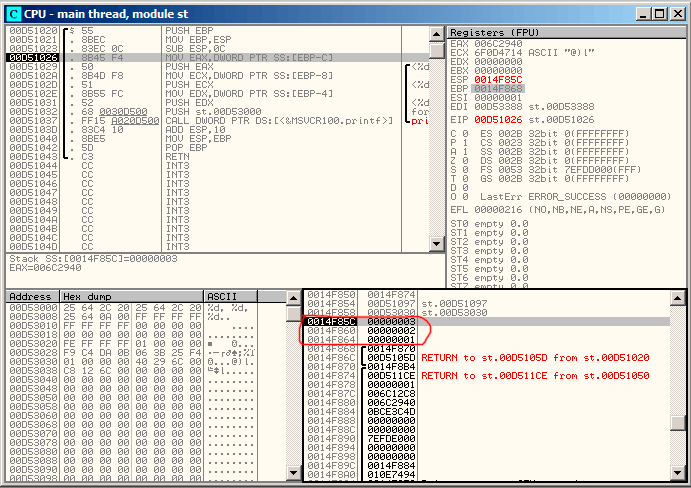
\includegraphics[scale=\FigScale]{\CURPATH/olly2.png}
\caption{\olly: \RU{последний вызов \ttf{}}\EN{last call of \ttf{}}}
\label{fig:fib_olly2}
\end{figure}

\RU{Теперь переменная \IT{next} присутствует в каждом фрейме.}
\EN{Now the \IT{next} variable is present in each frame.}

\clearpage
\RU{Рассмотрим стек более пристально. Я снова добавил туда своих комментариев}
\EN{Let's investigate the stack more closely. I have added my comments again}:

\lstinputlisting{\CURPATH/stack2.txt.\LANG}

\RU{Значение переменной \IT{next} вычисляется в каждой инкарнации функции, затем передается
аргумент $b$ в следующую инкарнацию} % FIXME what a word! hmmm...
\EN{Here we see it: the \IT{next} value is calculated in each function incarnation, then passed as
argument $b$ to the next incarnation}.

\section{\RU{Итог}\EN{Summary}}

\label{Recursion_and_tail_call}
\index{\Recursion}
\RU{Рекурсивные функции эстетически красивы, но технически могут ухудшать производительность
из-за активного использования стека}
\EN{Recursive functions are \ae{}sthetically nice, but technically may degrade performance because
of their heavy stack usage}.
\RU{Тот, кто пишет критические к времени исполнения участки кода, наверное, должен избегать 
применение там рекурсии}\EN{Everyone who writes performance critical code probably should
should avoid recursion}.

\RU{Например, однажды я написал функцию для поиска нужного узла в двоичном дереве. 
Рекурсивно она выглядела очень красиво, но из-за того, что при каждом вызове тратилось время на эпилог и пролог, 
все это работало в несколько раз медленнее чем та же функция, но без рекурсии.}
\EN{For example, I once wrote a function to seek a particular node in a binary tree. 
As a recursive function it looked quite stylish but since additional time
was to be spent at each function call
for the prologue/epilogue, it was working a couple of times slower than an iterative (recursion-free)
implementation.}

\newcommand{\FnFP}{\footnote{LISP, Python, Lua, \etc{}.}}
\index{\Recursion!Tail recursion}
\RU{Кстати, поэтому некоторые компиляторы функциональных \ac{PL}\FnFP{} (где рекурсия активно применяется) используют \glslink{tail call}{хвостовую рекурсию}.}
\EN{By the way, that is the reason some functional \ac{PL}\FnFP{} compilers (where recursion is used heavily) use \gls{tail call}.}
\fi % \IncludeOlly
